\chapter{Visão Geral}

Para embasar e planejar o projeto a ser desenvolvido, uma proposta de
arquitetura precisa ser feito. Neste capítulo será apresentado a proposta do projeto UMISS,
sendo explanado as arquiteturas de cada subsistema.

\section{Subsistema - Processamento de Sinais e Monitoramento}

O subsistema de controle e monitoramento terá como grande objetivo a aquisição
dos sinais do paciente, a disponibilização desses recursos para os
interessados, e a notificação dos responsáveis em casos de eventos críticos.
Sua arquitetura pode ser dividido em três grandes
módulos: o módulo que chamaremos \textbf{módulo eletrônico}, que conterá
grande parte dos componentes eletrônicos do projeto,
o \textbf{módulo servidor remoto}, que será um servidor remoto disponível
para ser consumido por outros serviços, e o \textbf{módulo aplicativo},
que será uma solução em aplicativo para ser utilizado pelos interessados.

\subsection{Módulo Eletrônico}
O módulo eletrônico será composto principalmente por sensores, amplificadores,
filtros, conversores, e um sistema embarcado.

Os sensores terão como principal papel a extração dos sinais vitais do
paciente, e serão acoplados a estrutura da cadeira, de forma que algum
membro do paciente fique em contato com o sensor, permitindo assim a
aquisição do sinal.

Os amplificadores e filtros serão responsáveis pelo condicionamento do sinal. 
Os sinais adquiridos serão amplificados, por tratarem-se de sinais de baixa 
amplitude, e filtrados para atenuação de ruídos de frequências indesejadas.

Os conversores DAC (\textit{Digital Analog Converter}) terão como papel a conversão 
dos sinais analógicos adquiridos do usuário para formato digital, para que
possam ser processados pelo processador central do sistema.

Um sistema embarcado será responsável por receber os sinais do paciente,
processá-los e utilizá-los em tarefas específicas, e, por fim, despachar os
dados para o módulo servidor remoto.

\subsection{Módulo Servidor Remoto}
O módulo servidor remoto é dividido nos seguintes componentes: um servidor remoto
e gerência de configuração do servidor.

O servidor remoto será um servidor hospedado fora da rede-interna da parte
eletrônica, e poderá ser acessado via \textit{internet}. Se comunicará com
o sistema embarcado da parte eletrônica utilizando comunicação
\textit{via socket}\footnote{\url{https://docs.oracle.com/javase/tutorial/networking/sockets/definition.html}},
apresentará dados para o aplicativo, e o notificará da ocorrência de eventos
críticos.

A gerência de configuração do servidor será composta principalmente de
configurações e \textit{scripts} que vão permitir a manutenção e
interoperabilidade entre o servidor e outros recursos.

\subsection{Módulo aplicativo}

O aplicativo só tem si próprio como componente, e será utilizado regularmente
pelos responsáveis do paciente; estará preparado para receber as notificações
do servidor e para mostrar os dados em tempo real.

\subsection{Integração entre os módulos}

\begin{figure}[H]
  \centering
    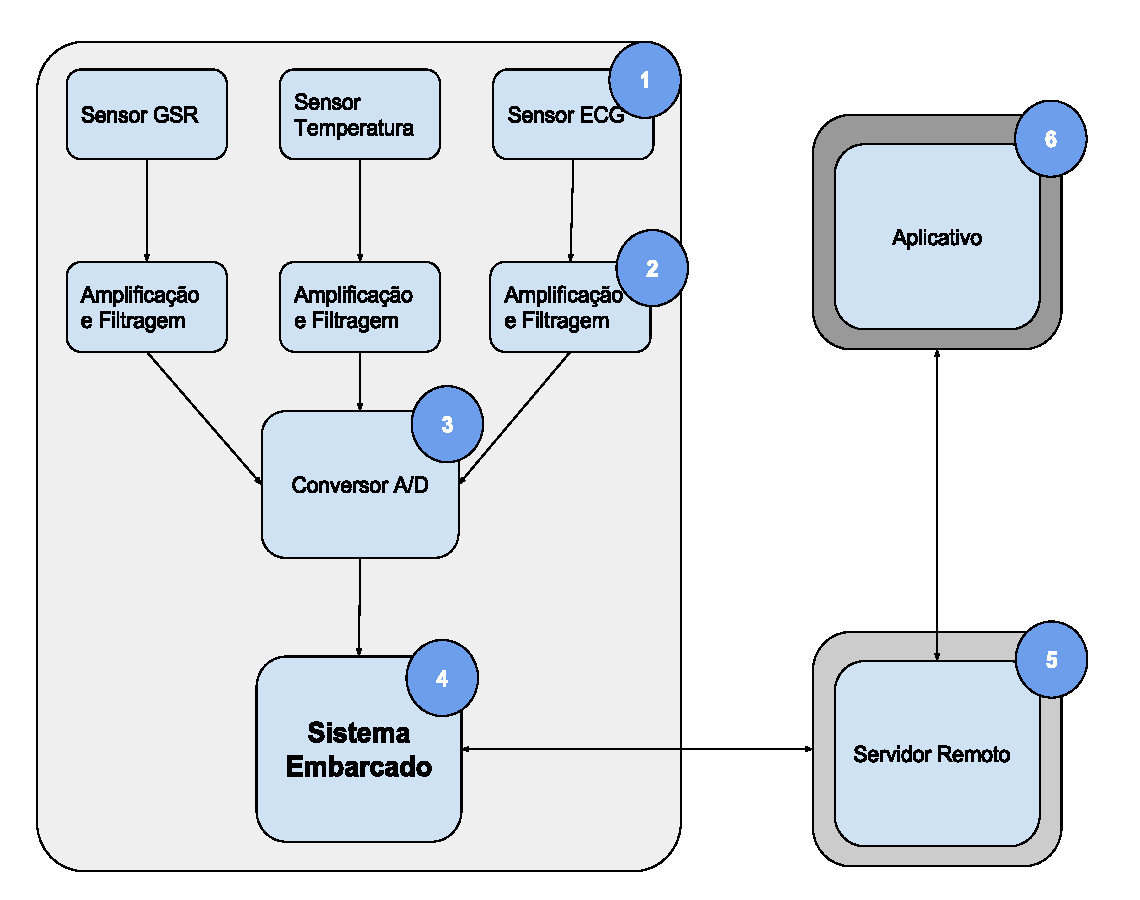
\includegraphics[width=\textwidth]{figuras/arquitetura-monitoramentoecontrole.eps}
  \caption{Fluxo típico do subsistema de Monitoramento e Controle}
  \label{fig:arquitetura-monitoramento-e-controle}
\end{figure}

O passo (1) do subsistema é atuado pelos sensores, que extraírão sinais do paciente;
o passo (2) será atuado pelos amplificadores e filtros, e tratarão o sinal
extraído pelos sensores no passo anterior; no passo (3) os sinais tratados
são convertidos para formato digital, para que possam ser lidos pelo sistema
embarcado; no passo (4) o sistema embarcado recebe as informações do conversor
e abre conexão com o servidor remoto - após, envia as informações recebidas,
quando necessário; no passo (5) o servidor remoto recebe dados do sistema
embarcado e passa informações importantes para o aplicativo, e, por fim,
no passo (6), o aplicativo recebe as informações.

\subsection{Tecnologias Utilizadas}

\subsubsection{Servidor Django}
\label{sub:servidor_django}
O passo (5), retratado na Figura \ref{fig:arquitetura-monitoramento-e-controle},
representa o servidor remoto, que irá receber as informações de todas as
estações embarcadas do sistema. Este será responsável por receber, processar
e se comunicar com os dispositivos móveis cadastrados no sistema. Para tal,
será utilizado uma linguagem de programação compatível com a que será utilizada
no software embarcado, que será escrito em python. Desta maneira, todo
o servidor proverá serviços utilizando python.

Um Framework robusto e já bastante consolidado na comunidade python é o Django.
Este é bem completo e possui várias ferramentas que auxiliam no desenvolvimento.
O django possui um framework para API's Rest, que será o padrão utilizado pelos
clientes para se comunicarem, chamado de DjangoRestFramework. Este é muito poderoso
e de alta produtividade.

Estas três ferramentas irão compor juntas o passo (5).

\subsubsection{Sistema Embarcado}
Um sistema central de processamento foi selecionado para compor o passo (4).
A placa de desenvolvimento Raspberry Pi 3 Model B, apresentada na Figura \ref{rasp} foi selecionada para
a execução do processamento dos dados adiquiridos por possuir, além de alta 
velocidade de processamento, conexão WiFi, o que possibilita a comunicação 
com o servidor remoto, de acordo com os requisitos do projeto.

\begin{figure}[H]
  \centering
    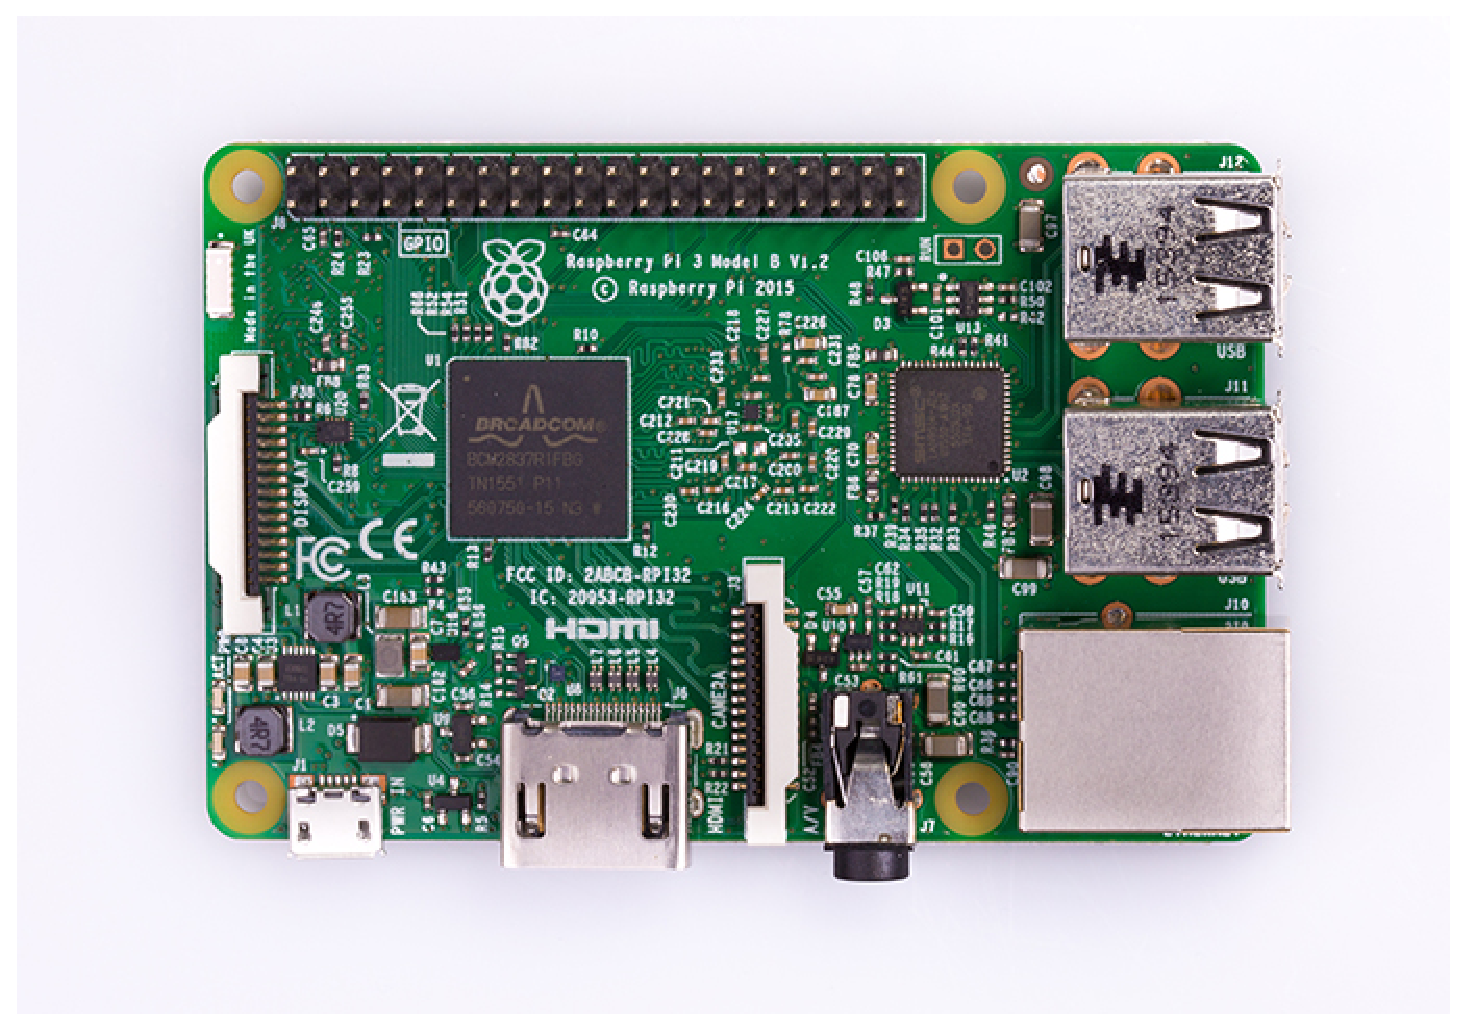
\includegraphics[keepaspectratio=true,scale=0.6]{figuras/rasp.eps}
  \caption{Microcomputador Raspberry Pi 3 Modelo B.}
  \label{fig:rasp}
\end{figure}

\subsubsection{Conversor AD}
Para a conversão dos sinais analógicos para digitais, foi selecionado o conversor 
AD ADS1115, apresentado na Figura \ref{ads}, que possui quatro canais de entrada analógica, resolução de 16 bits 
e amostragem de 800Hz. 

\begin{figure}[H]
  \centering
    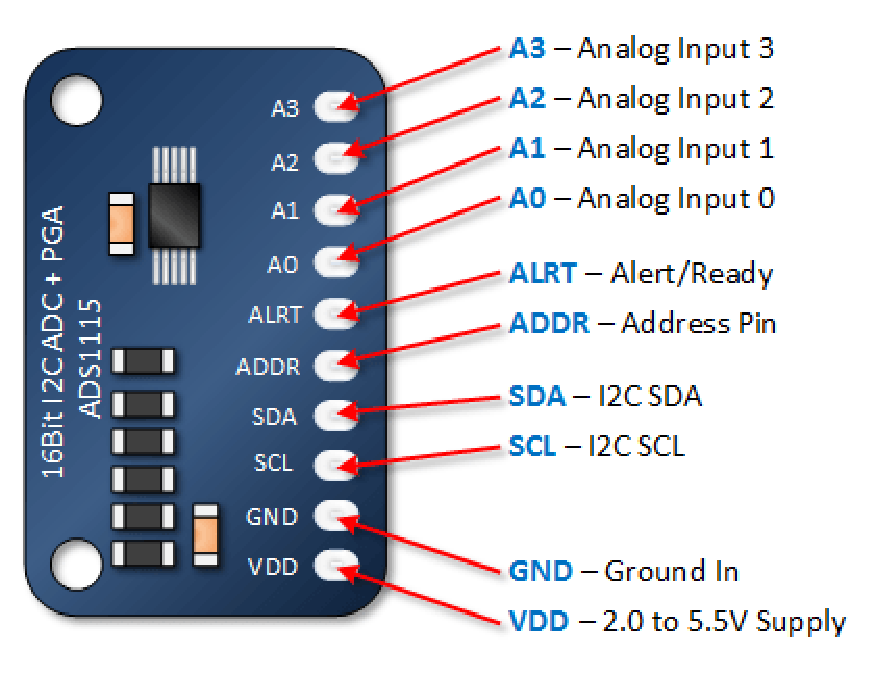
\includegraphics[keepaspectratio=true,scale=0.7]{figuras/ads.eps}
  \caption{Conversor analógico-digital ADS1115.}
  \label{fig:ads}
\end{figure}

Preocupações de importante ressalte durante a seleção do 
conversor 
foram sua resolução e amostragem. O conversor ADS1115 possui alta 
resolução com 
seus 16 bits, possibilitando uma captura mais refinada dos sinais 
de pequena 
variação. Além disso, possui amostragem de 800Hz, necessária 
para captura 
de sinais de eletrocardiograma (ECG) e frequência cardíaca, 
que possuem 
frequências úteis até 300Hz, dessa forma, 800Hz de amostragem 
mostra-se 
suficente para boa captura desses sinais, entre os outros necessários para o projeto.

\subsubsection{Amplificadores de Intrumentação e Operacionais}
Para os sistemas de amplificação dos sinais capturados e condicionamento dos mesmos, serão utilizados amplificadores operacionais e de intrumentação.

A amplificação e captura de sinais vitais de baixa amplitude de forma ótima é 
uma tarefa que requer um amplificador de instrumentação, com ganho regulável 
por divisores de tensão, permitem aplicação de alto ganho sem aplicar novos 
ruídos ao sinal. Para a amplificação dos sinais para frequência cardíaca 
serão utilizados amplificadores INA118 e INA128, fabricados pela \textit{Texas Instruments}. Além, para a filtragem dos sinais, serão implemetadas 
topologias de filtragem analógica do tipo \textit{Sallen-Key}, que necessitam da 
utilização de amplificadores operacionais para seleção das frequências 
de corte desejadas, para estes, serão utilizados amplificadores TL084, 
da \textit{Texas Instruments}, por maior concentração de amplificadores 
por chip e pelo baixo ruído apresentado por estes amplificadores.

\subsubsection{Aquisição de Sinais}
Para a aquisição dos sinais do usuário, serão utilizados sensores e eletrodos específicos para cada tipo de sinal. Para a captura dos sinais de resistência galvânica da pele (GSR), pela qual é possível identificar alterações de estresse do usuário e prováveis convulsões ou crises hipoglicêmicas, serão utilizados eletrodos com contatos de prata ou alumínio, em contato com os dedos ou pulso do usuário.

Para a aquisição dos sinais de temperatura corporal, serão utilizados termistores, que consistem em resistores que apresentam variação de resistência para variações de temperaturas, regidas pela equação de \textit{Steinhart-Hart} \cite{gregg}, para esses termistores, haverão, no sistema embarcado, rotinas para definir a temperatura corporal a partir de valores de tensão recebidos.

Além, para captura de sinais de frequência cardíaca, serão utilizados sensores ópticos ou eletrodos de contato para captura dos sinais de eletrocardiograma (ECG).

Na Figura \ref{sensors} é possível visualizar modelos comuns dos sensores e eletrodos utilizados.

\begin{figure}[H]
  \centering
    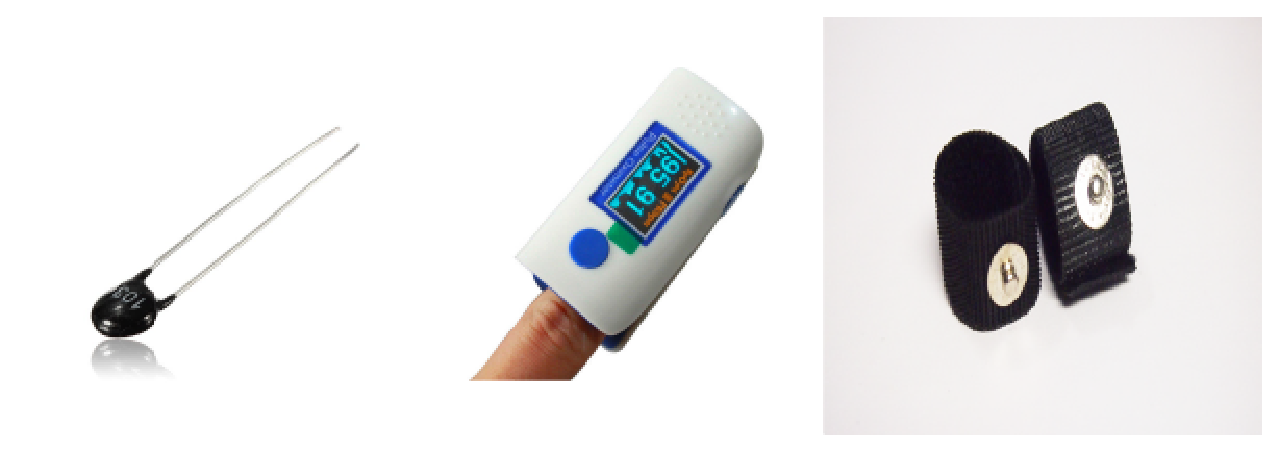
\includegraphics[width=\textwidth]{figuras/sensors.eps}
  \caption{Sensores e eletrodos para captura de sinais: Termistor NTC 10K para temperatura, oximetro de dedo para frequência cardíaca e contatos de prata para captura de GSR.}
  \label{fig:sensors}
\end{figure}

\section{Subsistema - Controle e Alimentação}
\subsection{Dimensionamento de Motores e Sistema Energético}
Neste projeto serão usados motores de corrente contínua a fim de movimentar o conjunto
cadeira $+$ paciente, esses motores devem ser capazes de fornecer o torque solicitado
nas diversas situações, como o uso com carga elevada e a movimentação em aclives.
Serão usados circuitos driver para o controle de tais motores. De forma simplificada
uma máquina de corrente contínua é formada por duas partes distintas, a parte
estacionária chamada de estator, onde estão localizados os polos indutores e o
enrolamento de campo, e a parte girante chamada de rotor onde se encontram as
bobinas do enrolamento de armadura, bem como o comutador  \cite{bim}. O comutador
é um conjunto de barras isoladas entre si e conectadas no eixo do rotor, ele tem
a função de mudar o sentido da corrente que passa pelo enrolamento de armadura.
Um exemplo de rotor e estator é mostrado na figura~\ref{fig:rotor}.

\begin{figure}[H]
  \centering
    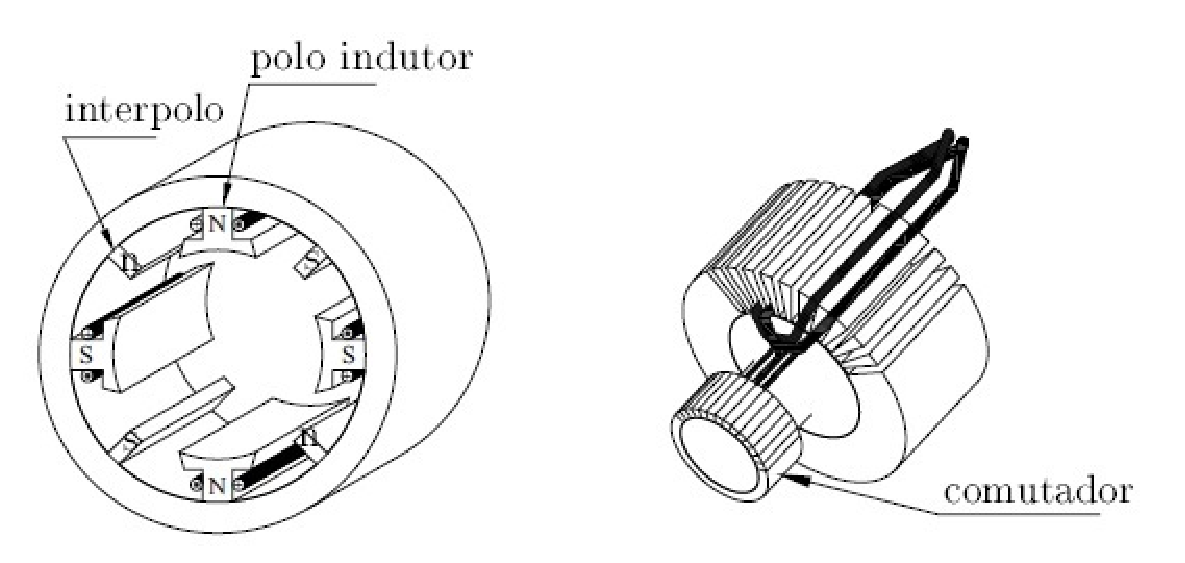
\includegraphics[width=\textwidth]{figuras/rotor.eps}
  \caption{Exemplo de um estator e um rotor \cite{bim}}
  \label{fig:rotor}
\end{figure}

\subsubsection{Dimensionamento do Sistema Eletromecânico}

Para a análise das características requeridas de torque e potência foram estimados
massa do 
sistema foi estimada como $150 kg$, a sua velocidade máxima 
como $3 km/h$
e o tempo para atingir tal velocidade como $4$ segundos. 
A partir desses dados é
possível 
calcular a força necessária para colocar a cadeira em movimento 
bem como
para a acelerar até a velocidade máxima. Dividindo a velocidade pelo tempo necessário
para se alcançar a velocidade é possível calcular a aceleração.

\begin{equation}
a = \frac{V}{t} = \frac{3}{3,6\cdot 4} = 0,20834  \frac{m}{s^2}
\end{equation}

Em seguida calculamos a força necessária para acelerar a massa de $150 kg$.

\begin{equation}
F_{a} = M \cdot a = 150 \cdot 0,20834 = 31,25 N
\end{equation}

Também deve ser levado em conta a força necessária para colocar 
a massa da cadeira
em movimento, 
e usamos um valor de coeficiente de atrito estático $\varsigma_{a} = 0,3$.

\begin{equation}
F_{r} = M \cdot g \cdot \varsigma_{a} = 441,45 N
\end{equation}

Então, a força total solicitada para que a cadeira seja movida 
em um plano 
horizontal e liso é dada pela soma da força de resistência ao 
movimento e da força de aceleração.

\begin{equation}
F_{T} = F_{a} + F_{r} = 472,7 N
\end{equation}

Finalmente é possível calcular o torque solicitado utilizando o raio do eixo do
motor de $4mm$.

\begin{equation}
T = F_{T} \cdot R = 472,7 \cdot 0,004 = 1,8908 N\cdot m
\end{equation}

A potência requerida é calculada multiplicando-se a força pela velocidade máxima.

\begin{equation}
P = F_{T} \cdot V = 472,7 \cdot 0,83334 = 393 W
\end{equation}

Diante disso, o dimensionamento acima foi feito para que o 
movimento da cadeira se dê em um plano horizontal e liso. 
Para que a cadeira se movimente em rampas é necessário considerar 
a inclinação das mesmas nos cálculos, para isso a Norma ABNT NBR 9050 \cite{nbr9050}
estipula a inclinação máxima que rampas de acessibilidade 
podem ter, que é de aproximadamente 8°. Assim, adotando que a velocidade 
máxima alcançada pela cadeira em aclives seja de 2 km/h, tem-se o 
dimensionamento da aceleração para essa situação: 

\begin{equation}
a = \frac{V}{t} = \frac{2}{3,6 \cdot 4} = 0,1389 \frac{m}{s^2}
\end{equation}

Então a força total solicitada para que a cadeira seja movida 
em um plano inclinado de 8° é dada pela soma da força de resistência 
ao movimento e da força de aceleração, e ainda a força referente a inclinação do piso:

\begin{equation}
F_{T} = F_{r} + F_{a} + F_{i} = [\varsigma_{a} \cdot M \cdot g \cdot cos(8º)] + [M_{a}] + [M \cdot g \cdot sin(8º)]
\end{equation}

\begin{equation}
F_{T} = [0,3 \cdot 150 \cdot 9,81 \cdot cos(8º)] + [150 \cdot 0,1389] + [150 \cdot 9,81 \cdot sin(8º)]
\end{equation}

\begin{equation}
F_{T} = 643,2319 N
\end{equation}

Com isso é possível calcular o torque solicitado utilizando o raio do eixo do motor de 4mm.

\begin{equation}
T = F_{T} \cdot R = 643,2319 \cdot 0,0004 = 2,5729 N \cdot m
\end{equation}

A potência requerida é calculada multiplicando-se a força total pela velocidade máxima.

\begin{equation}
P = F_{T} \cdot V = 643,2319 \cdot 0,55556 = 357,35 W
\end{equation}

\subsubsection{Especificações do Motor}

Serão utilizados dois motores Bosch modelo GPB F006 KM0 611, que tem aplicações
em sistemas de arrefecimento, o emprego dos dois motores satisfaz as exigências
de potência e torque do sistema. As curvas características desse motor e seus
dados técnicos são mostrados a seguir.

\begin{figure}[H]
  \centering
    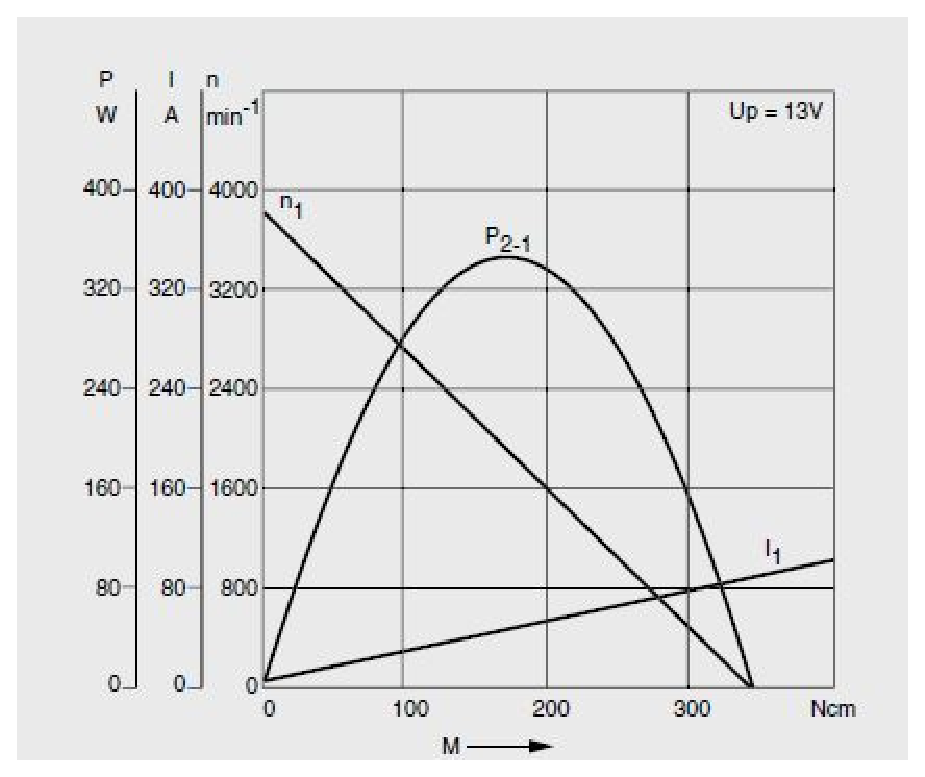
\includegraphics[width=\textwidth]{figuras/motor.eps}
  \caption{Curvas de motor GPB F006 KM0 611 (Bosch)}
  \label{fig:motor}
\end{figure}

\begin{table}[h]
\centering
\vspace{0.5cm}
\begin{tabular}{|l|l|}
\hline
Item                & Especificação \\
\hline
Tensão Nominal      & 12 V \\
Potência Nominal    & 305 W \\
Rotação Nominal     & 2600 rpm \\
Corrente Nominal    & 25A \\
Torque Nominal      & 350 Ncm \\
Peso                & 1,585 kg \\
\hline
\end{tabular}
\caption{Dados motor GPB F006 KM0 611 (Bosch)}
\label{tab:dadosmotor}
\end{table}

Como foram selecionados dois motores, é válido ressaltar 
que os valores de torque e potência dimensionados acima deverão ser divididos por dois.


\subsubsection{Dimensionamento da Bateria}

Sabe-se que a potência necessária para movimentar a cadeira de rodas é de $367 W$,
também sabe-se que a tensão nominal do motor GPB F006 KM0 611 da Bosch é de $12V$,
logo as baterias devem ser capazes de fornecer essa potência para o sistema por
pelo menos 3 horas. Para determinar qual bateria usar deve ser estimada a
capacidade em Ah, também devem as suas dimensões e peso, outro fator importante
é o custo, já que o projeto tem orçamento limitado \cite{costa}.

A bateria a ser utilizada deve ter uma tensão de $12V$, pois esse valor é
compatível tanto com a necessidade dos motores quanto com a disponibilidade dos
modelos de mercado. Tendo em vista a potência calculada e a tensão estabelecida
é possível calcular a corrente necessária.

\begin{equation}
P = V \cdot I
\end{equation}

\begin{equation}
I = \frac{393}{12} = 32,75 A
\end{equation}

Com esse valor de corrente e o tempo de trabalho do sistema é possível calcular
a carga da bateria.

\begin{equation}
C = I \cdot t = 32,75 \cdot 3 = 98,25 Ah
\end{equation}

Sabe-se que a bateria não deve ser totalmente descarregada, pois isso diminui a
vida útil da mesma, logo deve ser utilizado um fator de profundidade de descarga,
que nesse caso será de $80\%$ \cite{KARASINSKI}.

\begin{equation}
C = \frac{98,25}{0,8} = 122,125 Ah
\end{equation}

Um ponto importante no dimensionamento é o fato de o sistema de movimentação não
operar em plena carga a todo tempo, havendo momentos em que a potência necessária
é reduzida ou até mesmo nula, situação onde a cadeira está parada, portanto deve
se estimar um fator de demanda para os motores, para esse projeto o valor
adotado de para o fato de demanda será de $0,75$. Com isso temos que a carga
necessária será de:

\begin{equation}
C = 122,125 \cdot 0,75 = 92,1Ah
\end{equation}

Uma possível solução que prioriza a variável custo é a utilização de $3$ baterias
de chumbo-ácido de $30 Ah$ ligadas em paralelo.

\subsection{Sistema de Controle de Movimento}
Para o acionamento dos motores tem-se duas variáveis que devem 
ser consideradas, o controle da velocidade e do torque desses 
motores, de forma que o sistema de acionamento propicie ao usuário 
uma experiência de segurança e conforto. Com o enfoque nesse sentido, 
a arquitetura proposta está em fazer o acionamento dos motores de 
maneira unilateral, isto é, fazer o acionamento de cada motor 
individualmente, tendo um controle melhor da velocidade e torque 
proporcionados às rodas através dos motores.

Os componentes para movimentação da cadeira de rodas, além 
dos motores, são o joystick, um microcontrolador e um circuito 
de ponte H. Esses componentes juntamente com os motores proporcionam 
a movimentação da cadeira e suas funções podem ser entendidas 
pelos seguintes passos, mostrados na Figura \ref{fig:control_arch}.

\begin{figure}[H]
  \centering
    \includegraphics[width=\textwidth]{figuras/control_arch.eps}
  \caption{Fluxo típico do sistema de controle e movimentação dos motores.}
  \label{fig:control_arch}
\end{figure}

\begin{enumerate}
\item O  joystick, acoplado ao braço da cadeira, 
mandará sinais de direção para um microcontrolador;
\item O microcontrolador então gerará os sinais de 
PWM necessários e os enviará para um circuito de ponte H;
\item A ponte H acionará os motores com o controle de 
tensão adequado orientando a direção e intensidade definidas pelo sinal PWM.
\end{enumerate}

A direção de movimento da cadeira depende da intensidade 
da corrente em cada motor. Para se andar em direção reta, 
ambos os motores devem possuir a mesma corrente, com a direção 
da mesma determinando o sentido de rotação dos motores. Para se 
fazer uma curva, um dos motores deve estar mais rápido, ou seja, 
com corrente maior que o outro. Portanto, com a definição 
dos motores e suas características, tais como corrente nominal, 
tensão nominal e potência nominal, conseguimos dimensionar 
a ponte H para que estabeleça corretamente o nível de tensão que 
se deve chegar aos motores para a movimentação completa e segura da cadeira.

O \textit{joystick} a ser utilizado será um \textit{joystick} 
de três eixos, apresentado na Figura \ref{fig:joystick}. Seu funcionamento é dado através do controle de 
dois potenciômetros e um botão, sendo que os eixos X e Y são 
correspondentes às entradas dos potenciômetros e o eixo Z corresponde ao botão quando pressionado.

\begin{figure}[H]
  \centering
    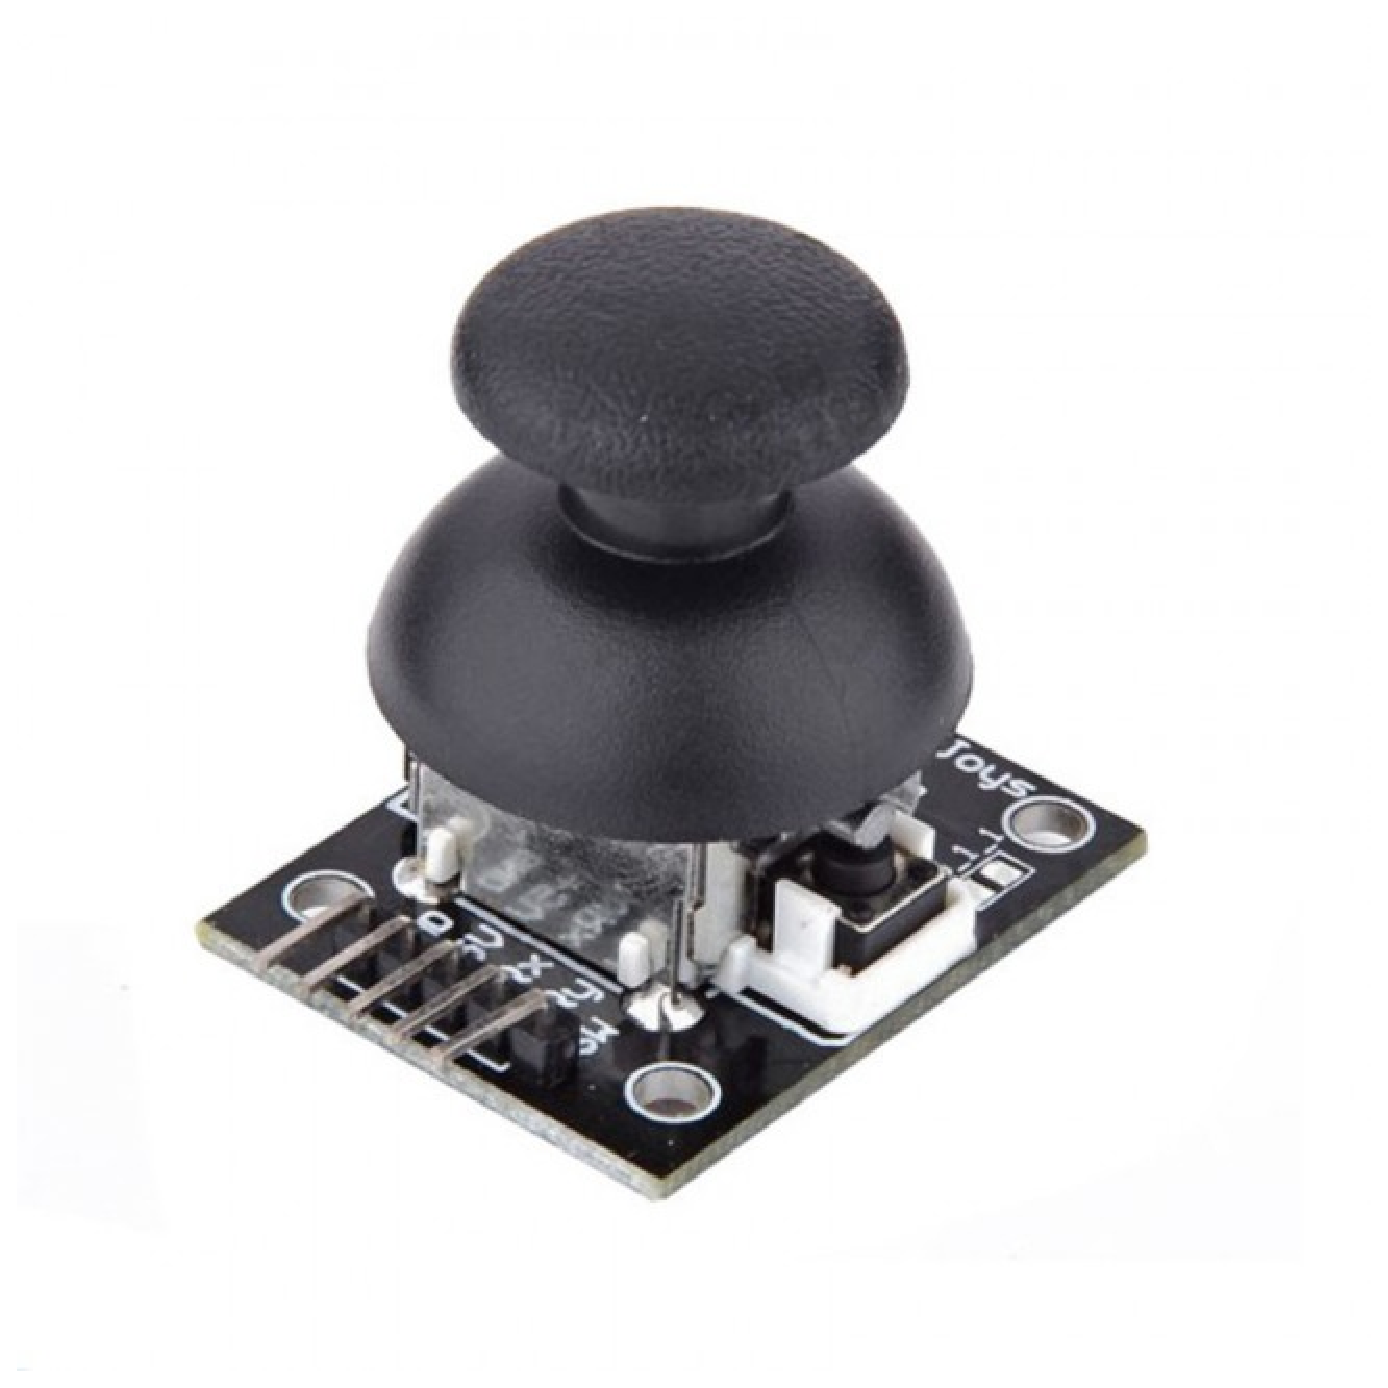
\includegraphics[width=\textwidth]{figuras/joystick.eps}
  \caption{\textit{Joystick} de três eixos para controle de velocidade e direção da cadeira.}
  \label{fig:joystick}
\end{figure}

O microcontrolador a ser utilizado para receber as informações 
do joystick e gerar os sinais de PWM para a movimentação 
da cadeira será o Arduino UNO com processador ATmega328, mostrado na Figura \ref{fig:arduino}. A escolha deste 
microcontrolador se deve por ser um microcontrolador que o grupo 
já possui e por ser um microcontrolador de leitura e escrita de 
sinais já dominados pelos integrantes do grupo, tornando-a 
uma ferramenta de confiabilidade adequada ao projeto. O Arduino UNO
possui a possibilidade de se controlar a frequência que se deseja 
para os sinais 
PWM através de três timers que se encontram no ATmega 328, o que nos 
dá a flexibilidade dos níveis de tensão que serão enviados ao 
circuito de ponte H e do controle dos motores.

\begin{figure}[H]
  \centering
    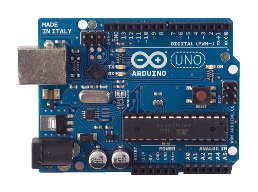
\includegraphics[width=\textwidth]{figuras/arduino.eps}
  \caption{Arduino UNO com processador ATmega 328.}
  \label{fig:arduino}
\end{figure}

A ponte H, responsável pelo controle de sentido de rotação e 
potência para o motor, possui em sua configuração quatro 
transistores FET de potência. Sua funcionalidade depende 
da polarização dos transistores que determina o sentido da corrente 
que vai passar pelo motor, acionando o motor no sentido que se deseja. 
Por exemplo, polarizando-se os transistores Q1 e Q4, apresentados 
na Figura \ref{fig:ponte_h}, a corrente vai passar pelo motor no 
sentido esquerda-direita e para o sentido direita-esquerda 
polariza-se os transistores Q2 e Q3. Portanto, tendo em mãos as 
características dos motores a serem utilizados, consegue-se 
dimensionar a ponte H de tal forma que a mesma consiga ter o 
controle da corrente que vai passar pelo motor. Os transistores 
de potência que serão utilizados para montagem da ponte H serão do 
modelo IRF3505 de canal N, que segundo seu datasheet suporta uma 
corrente de $71$ A em seu limite de temperatura de encapsulamento, 
sendo o suficiente para controle do motor, visto que o mesmo 
possui uma corrente de operação nominal de $25$ A.

\begin{figure}[H]
  \centering
    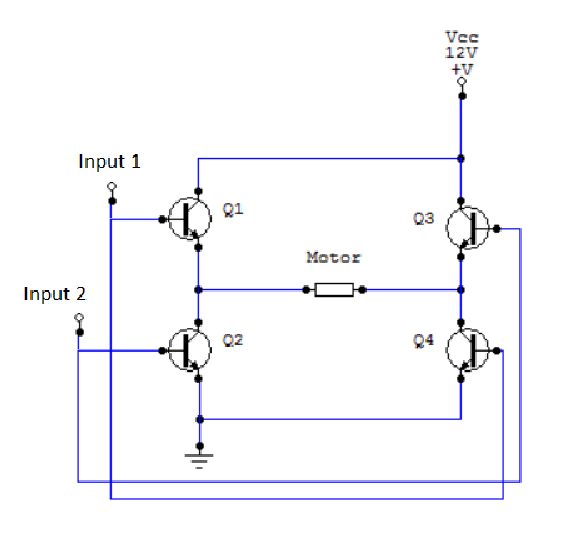
\includegraphics[width=\textwidth]{figuras/ponte_h.eps}
  \caption{Esquemático de sistema de Ponte H com transistores para controle de sentido de rotação dos motores.}
  \label{fig:ponte_h}
\end{figure}

\section{Subsistema - Projeto Estrutural}
O Subsistema de estrutura será dividido em dois elementos: 
Elemento Estrutural da Cadeira de Roda e Elemento de Transmissão 
que conduz o torque do motor para as rodas da Cadeira.

Nesse subconjunto estrutural, os componentes do projeto irão 
manufaturar uma Cadeira de Roda de maneira que possa sustentar 
os componentes como motores, baterias, sensores e até mesmo o 
usuário. Para isso será utilizado \textit{Sketchs} Manuais 
para encontrar saídas factíveis para a melhor execução do projeto, 
escolha de materiais, projetar o esquemático em 3D, 
utilização também de um software CAE para análises estática, 
modal e de fadiga.Será feito também um estudo ergonômico 
para que o usuário tenha completo conforto quando utilizar a 
cadeira, tanto ao sentar quanto ao apoiar a cabeça. Por fim a 
manufatura será executada de acordo com o material escolhido 
e com as técnicas que oferecem a estrutura mais próxima do ideal.

Já o subconjunto da Transmissão irá desempenhar a função de 
transformar o torque do motor utilizado em movimento \cite{cardoso}. 
Assim, com as especificações dos motores que serão utilizados 
será possível modelar ou adquirir uma caixa de redução pronta para 
entregar as rodas que serão utilizadas no projeto o movimento desejado.

\begin{figure}[H]
  \centering
    \includegraphics[width=\textwidth]{figuras/structure_arch.eps}
  \caption{Fluxogramas com tomadas de decisão para cada ponto: Estrutura e Transmissão.}
  \label{fig:structure_arch}
\end{figure}

Como apresentado na Figura \ref{fig:structure_arch}, no fluxograma à esquerda, o primeiro passo 
será a modelagem manual de um sketch para melhor visualização 
e maior facilidade para um Brainstorming visando a melhor ideia 
de Cadeira de roda ou Adquirir uma cadeira para adaptar. 
O segundo passo é a escolha do material, levando em consideração 
o custo-benefício e facilidade com a utilização das técnicas de 
usinagem e conformação mecânica. O terceiro e quarto passo será 
utilizar com o auxílio de softwares CAD/CAE ( ANSYS e CATIA V5R19) 
para validar a estrutura em ambiente computacional. O quinto também 
com o auxílio do CAD, será utilizado algumas normas para melhor 
aplicar as normas de ergonomia. Por fim, com todos os passos anteriores bem sucedido o último passo seria a concepção do 
trabalho completo, a manufatura da estrutura. Em paralelo, o fluxograma à direira da \ref{fig:structure_arch}, 
que visa estudar a possibilidade de modelar uma caixa de redução 
para entregar um movimento aceitável para a cadeira. Caso não seja 
possível a 
aquisição de uma caixa totalmente projetada, caso não seja possível, 
será inevitável a busca de alternativas para melhor utilização dos motores.

\section{Outros}

\subsection{Integração Contínua}
